\documentclass[12pt,a4paper]{article}

\usepackage{fontspec}
\setmainfont{Times New Roman}
\setmonofont{Consolas}
\usepackage[russian]{babel}
\usepackage[left=25mm,right=15mm,top=20mm,bottom=20mm]{geometry}
\usepackage{graphicx}
\usepackage{fancyvrb}
\usepackage{enumitem}
\usepackage{float}
\usepackage{pdflscape}
\usepackage[hidelinks]{hyperref}

\setlist{nosep}
\setlength{\parindent}{0pt}
\setlength{\parskip}{6pt}

\begin{document}
\sloppy

\begin{titlepage}
    \centering
    «Национальный исследовательский университет ИТМО»\\[6pt]
    Факультет программной инженерии и компьютерной техники

    \vfill

    {\Large Лабораторная работа №1}\\[8pt]
    по дисциплине «Информационные системы»\\[8pt]
    Вариант 12030

    \vfill

    \begin{flushright}
        Выполнил: студент группы P3319\\
        Абрамов Егор Денисович\\[12pt]
        Преподаватель:\\
        Лисицина Василиса Васильевна
    \end{flushright}

    \vfill

    Санкт-Петербург, 2026
\end{titlepage}

\section{Текст задания}

Реализовать информационную систему, которая позволяет взаимодействовать с объектами класса \texttt{Organization}, описание которого приведено ниже:

\begin{Verbatim}[frame=single,fontsize=\small]
public class Organization {
    private long id; // > 0, уникальное, генерируется автоматически
    private String name; // не null, не пустая строка
    private Coordinates coordinates; // не null
    private java.time.LocalDateTime creationDate; // не null, автоматически
    private Address officialAddress; // может быть null
    private Float annualTurnover; // может быть null, > 0
    private int employeesCount; // > 0
    private Long rating; // может быть null, > 0
    private String fullName; // может быть null
    private OrganizationType type; // может быть null
    private Address postalAddress; // не null
}
public class Coordinates {
    private float x; // > -577
    private int y;
}
public class Address {
    private String street; // не null
    private Location town; // может быть null
}
public class Location {
    private long x;
    private Float y; // не null
    private String name; // не null
}
public enum OrganizationType {
    COMMERCIAL, TRUST, PRIVATE_LIMITED_COMPANY, OPEN_JOINT_STOCK_COMPANY;
}
\end{Verbatim}

Разработанная система должна удовлетворять следующим требованиям:
\begin{itemize}
    \item Основное назначение информационной системы "--- управление объектами, созданными на основе заданного в варианте класса.
    \item Необходимо, чтобы с помощью системы можно было выполнить следующие операции с объектами: создание нового объекта, получение информации об объекте по ИД, обновление объекта.
    \item Выполнение операций по управлению объектами должно осуществляться на серверной части (не на клиенте), изменения должны синхронизироваться с базой данных.
    \item На главном экране системы должен выводиться список текущих объектов в виде таблицы (каждый атрибут объекта "--- отдельная колонка в таблице). При отображении таблицы должна использоваться пагинация (если все объекты не помещаются на одном экране).
    \item Нужно обеспечить возможность фильтровать/сортировать строки таблицы, которые показывают объекты (по значениям любой из строковых колонок). Фильтрация элементов должна производиться по неполному совпадению.
    \item Переход к обновлению (модификации) объекта должен быть возможен из таблицы с общим списком объектов и из области с визуализацией объекта (при ее реализации).
    \item При добавлении/удалении/изменении объекта, он должен автоматически появиться/\allowbreak исчезнуть/\allowbreak измениться в интерфейсах у других пользователей, авторизованных в системе.
    \item Если при удалении объекта с ним связан другой объект, связанные объекты должны быть связаны с другим объектом (по выбору пользователя), а изначальный объект удален.
    \item Пользователи должны иметь возможность просмотра всех объектов. Для модификации объекта должно открываться отдельное диалоговое окно. При вводе некорректных значений в поля объекта должны появляться информативные сообщения о соответствующих ошибках.
\end{itemize}

В системе должен быть реализован отдельный пользовательский интерфейс для выполнения специальных операций над объектами:
\begin{itemize}
    \item Вернуть количество объектов, значение поля \texttt{fullName} которых больше заданного.
    \item Вернуть массив объектов, значение поля \texttt{name} которых содержит заданную подстроку.
    \item Вернуть массив уникальных значений поля \texttt{rating} по всем объектам.
    \item Вывести 5 организаций с максимальным годовым оборотом.
    \item Найти среднее количество сотрудников для 10 крупнейших организаций по годовому обороту.
\end{itemize}
Представленные операции должны быть реализованы в качестве функций БД, которые необходимо вызывать из уровня бизнес-логики приложения.

Особенности хранения объектов:
\begin{itemize}
    \item Организовать хранение данных об объектах в реляционной СУБД (PostgreSQL). Каждый объект, с которым работает ИС, должен быть сохранен в базе данных.
    \item Все требования к полям класса (указанные в виде комментариев к описанию классов) должны быть выполнены на уровне ORM и БД.
    \item Для генерации поля \texttt{id} использовать средства базы данных.
\end{itemize}

Особенности взаимодействия с пользователем:
\begin{itemize}
    \item Система должна реагировать на некорректный пользовательский ввод, ограничивая ввод недопустимых значений и информируя пользователей о причине ошибки.
    \item Переходы между различными логически обособленными частями системы должны осуществляться с помощью меню.
    \item При добавлении/удалении/изменении объекта, он должен автоматически появиться/\allowbreak исчезнуть/\allowbreak измениться на области у всех других клиентов.
\end{itemize}

Требования к реализации:
\begin{itemize}
    \item В качестве основы для реализации ИС необходимо использовать Jakarta EE, CDI beans.
    \item Для создания уровня хранения необходимо использовать EclipseLink.
    \item Разные уровни приложения должны быть отделены друг от друга, разные логические части ИС должны находиться в отдельных компонентах.
\end{itemize}

\section{UML-диаграммы}

Приложение построено по трёхслойной архитектуре: \texttt{handler} (REST-ресурсы JAX-RS) "--- \texttt{service} (бизнес-логика, CDI-бины) "--- \texttt{repository} (доступ к БД через EclipseLink). Обмен данными с клиентом идёт через DTO, уведомления об изменениях рассылаются через WebSocket, а коды HTTP-ответов выбирают мапперы исключений JAX-RS, так что сервисный слой не зависит от протокола.

\begin{figure}[H]
    \centering
    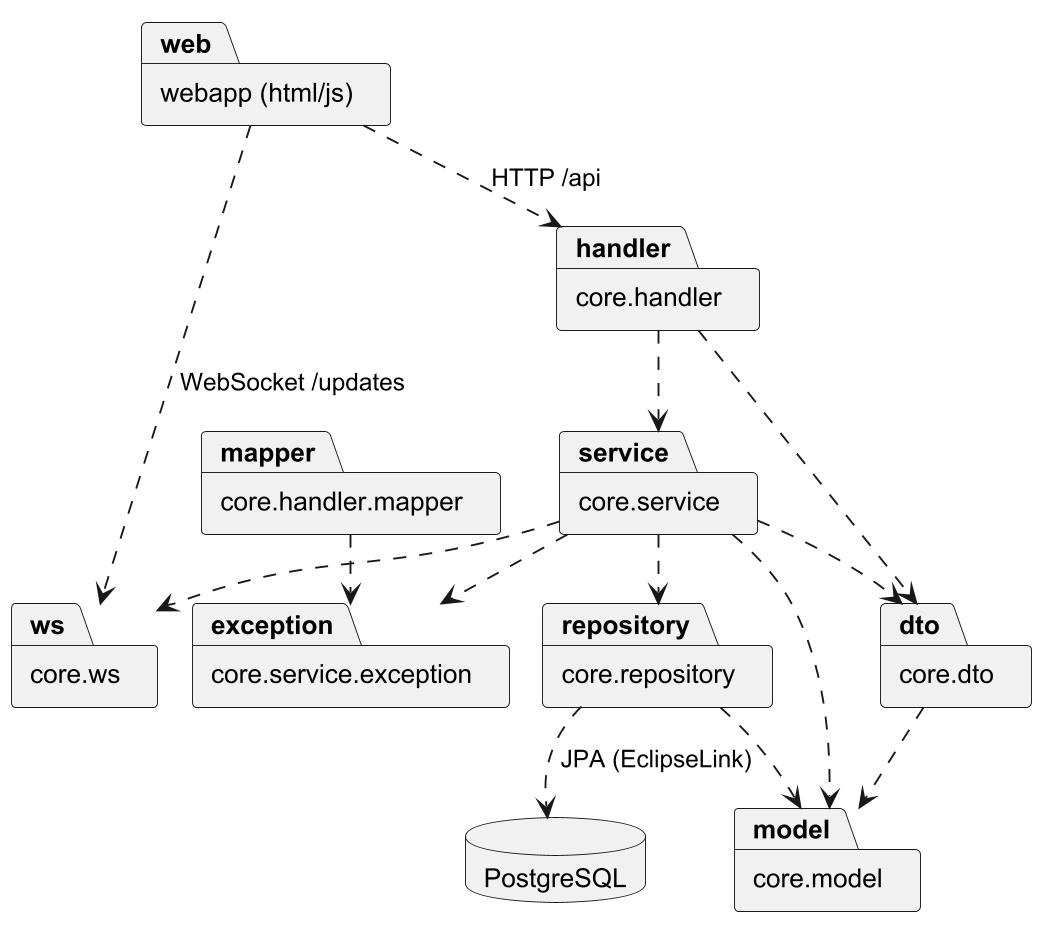
\includegraphics[width=0.7\textwidth]{img/packages.png}
    \caption{Диаграмма пакетов}
\end{figure}

\begin{figure}[H]
    \centering
    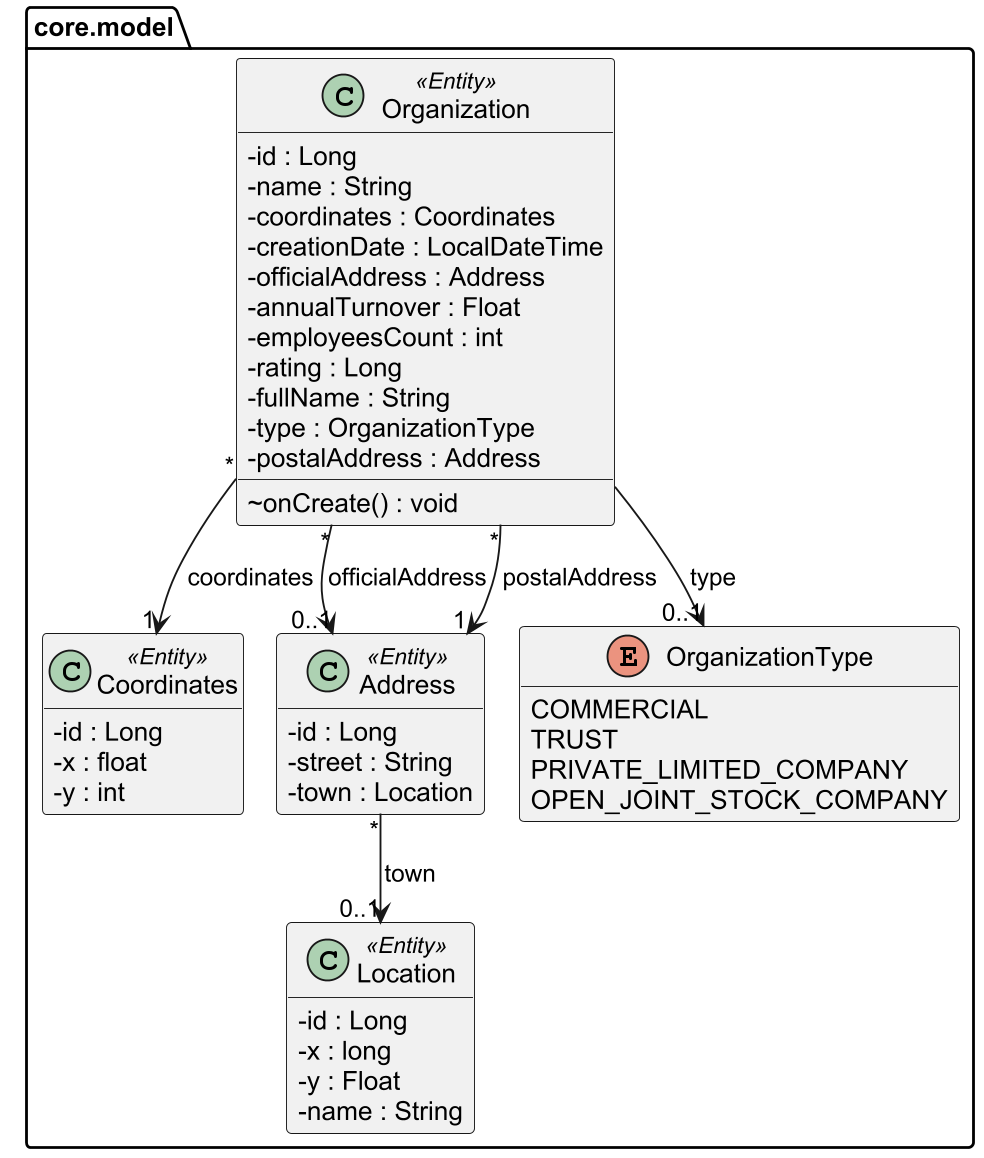
\includegraphics[width=0.75\textwidth]{img/model.png}
    \caption{Диаграмма классов модели}
\end{figure}

\begin{landscape}
\begin{figure}[H]
    \centering
    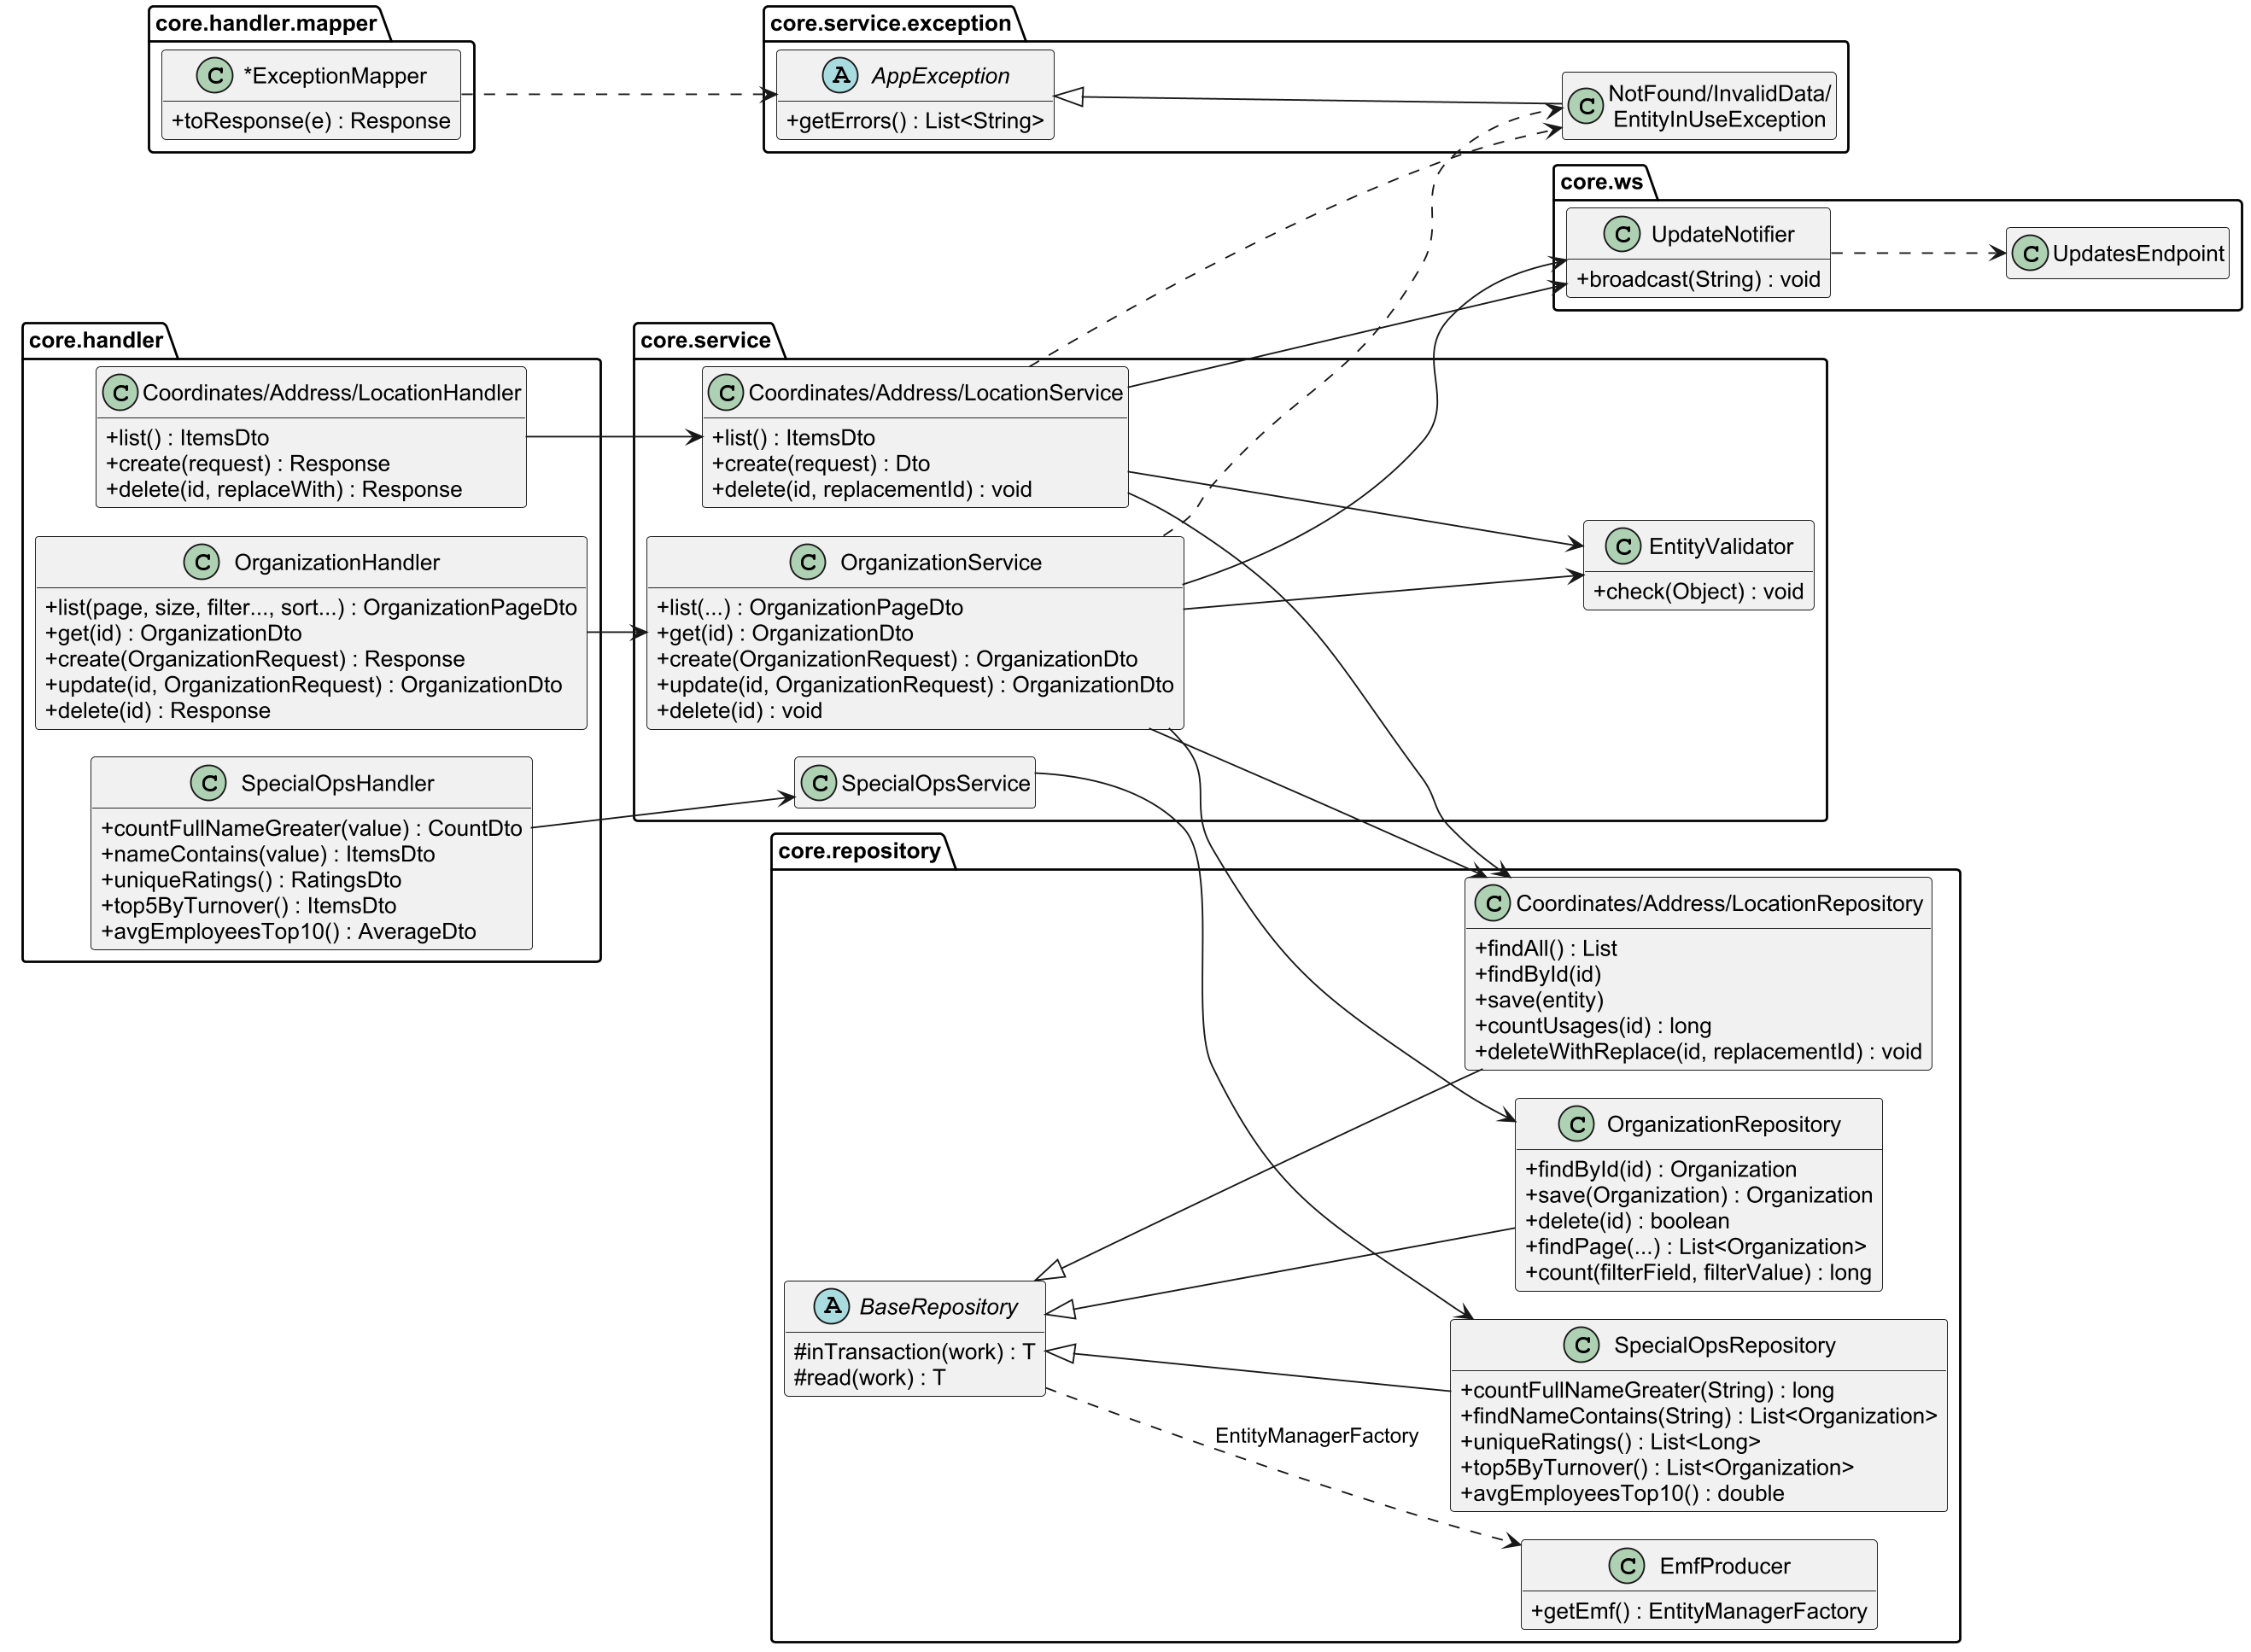
\includegraphics[width=\linewidth,height=0.9\textheight,keepaspectratio]{img/layers.png}
    \caption{Диаграмма классов слоёв приложения}
\end{figure}
\end{landscape}

\section{Исходный код}

Исходный код системы: \url{https://github.com/egor-abramov/IS-Lab-1/tree/main}

\section{Выводы}

В ходе работы была разработана информационная система для управления объектами \texttt{Organization} на платформе Jakarta EE. Уровень хранения реализован с помощью EclipseLink и PostgreSQL, ограничения на поля заданы и аннотациями Bean Validation, и ограничениями в таблицах БД, а специальные операции вынесены в функции БД. Изменения данных рассылаются всем клиентам через WebSocket. Были изучены CDI-бины, JAX-RS, технология Jakarta Persistence и её реализация EclipseLink, а также закреплено применение трёхслойной архитектуры.

\end{document}
